\chapter{Caminhos Mínimos em Grafos}

Neste capítulo estudamos o problema de encontrar caminhos de custo mínimo em grafos ponderados. 
Dado um grafo $G=(V,E)$ com pesos não negativos (ou, mais geralmente, reais) associados às arestas, queremos determinar o menor custo para alcançar cada vértice a partir de uma fonte $s$.

Esse problema aparece em contextos como:
roteamento em redes, planejamento de trajetos, logística, análise de dependências e muitos outros. 
Nos concentraremos nos algoritmos clássicos de caminhos mínimos a partir de uma única origem: \textbf{Dijkstra} e \textbf{Bellman--Ford}.

\subsection*{Caminhos e custo}

Um \textbf{caminho} em um grafo direcionado $G=(V,E)$ é uma sequência de vértices
\[
P = (v_0, v_1, \dots, v_k)
\]
tal que cada par consecutivo $(v_{i-1},v_i)$ é uma aresta do grafo:
\[
(v_{i-1},v_i) \in E \quad \text{para todo } i=1,\dots,k.
\]

O primeiro vértice $v_0$ é a \textbf{origem} do caminho e $v_k$ é o \textbf{destino}.
O número $k$ é o \textbf{comprimento} (em número de arestas).

Quando queremos enfatizar a origem e o destino, escrevemos
\[
P:\; s \leadsto v
\]
para indicar que $P$ é um caminho cujo primeiro vértice é $s$ e cujo último vértice é $v$.

Se cada aresta $(u,v)$ possui um peso ou custo $w(u,v)$, definimos o \textbf{custo do caminho} $P$ como
\[
w(P) = \sum_{i=1}^k w(v_{i-1},v_i).
\]

Entre todos os caminhos que ligam $s$ a $v$, a \textbf{distância mínima} (ou custo mínimo) é
\[
dist(s,v) = 
\min_{P:\, s \leadsto v} w(P).
\]

Se não existe nenhum caminho de $s$ até $v$, adotamos por convenção
\[
dist(s,v) = \infty.
\]

\medskip

\noindent
\textbf{Situações em que a distância mínima não existe.}
Se o grafo contém um \emph{ciclo de custo negativo} — isto é, uma sequência de vértices
\[
(v_0, v_1, \dots, v_k = v_0)
\]
tal que
\[
w(v_0,v_1) + \cdots + w(v_{k-1},v_0) < 0,
\]
e esse ciclo é alcançável a partir de $s$, então não existe distância mínima para certos vértices.
Isso ocorre porque podemos percorrer o ciclo negativo repetidas vezes, diminuindo
indefinidamente o custo total do caminho:
\[
w(P \circ \text{(ciclo)}^m) \longrightarrow -\infty.
\]

Nessas situações, não faz sentido falar em ``menor'' caminho, e algoritmos de caminhos mínimos
devem ser capazes de detectar a presença de ciclos negativos.
O algoritmo de Dijkstra não funciona quando há pesos negativos, enquanto o algoritmo de Bellman--Ford
detecta corretamente ciclos de custo negativo.

\subsection*{Árvore de caminhos mínimos}

Nos algoritmos apresentados aqui, além de calcular as distâncias, vamos construir uma 
\textbf{árvore de caminhos mínimos} enraizada em $s$.

\begin{itemize}
    \item Para cada vértice $v \neq s$, armazenamos uma aresta $(pai[v], v)$ que representa o último passo de um caminho mínimo de $s$ até $v$.
    \item O vértice $s$ é a raiz da árvore e satisfaz $pai[s] = s$.
    \item Percorrendo o vetor \texttt{pai[]} para trás (de $v$ até $s$), obtemos o caminho mínimo de $s$ até $v$.
\end{itemize}

Matematicamente, essa árvore é um subconjunto das arestas de $G$ com exatamente uma aresta saindo do pai de cada vértice $v \neq s$.  
Essa árvore não é conhecida a priori: iremos construí-la \textit{incrementalmente}, à medida que os algoritmos forem descobrindo novos caminhos mínimos.

\section{O Princípio do Relaxamento}

A operação central em algoritmos de caminhos mínimos é o \textbf{relaxamento} de arestas.  
Mantemos, para cada vértice $v$, uma estimativa $dist[v]$ do custo de um caminho de $s$ até $v$. 
Inicialmente, $dist[s] = 0$ e $dist[v] = \infty$ para $v \neq s$.

Dada uma aresta dirigida $(u,v)$ com peso $w(u,v)$, dizemos que \textbf{relaxamos} essa aresta quando executamos:

\[
\text{se } dist[v] > dist[u] + w(u,v)\text{, então}
\]
\[
dist[v] := dist[u] + w(u,v), \qquad pai[v] := u.
\]

Interpretando:

\begin{itemize}
    \item $dist[v]$ é sempre uma estimativa \emph{superior ou igual} à distância mínima real de $s$ até $v$;
    \item o relaxamento tenta melhorar essa estimativa, usando o caminho que passa por $u$;
    \item quando nenhum relaxamento é mais possível (de acordo com a estratégia do algoritmo), as estimativas se tornam exatamente as distâncias mínimas.
\end{itemize}

O vetor \texttt{pai[]} é atualizado junto com \texttt{dist[]} e registra a estrutura da árvore de caminhos mínimos: sempre que encontramos um caminho melhor para $v$, trocamos o pai de $v$.

Esse mesmo princípio será usado tanto no algoritmo de Dijkstra quanto no algoritmo de Bellman--Ford; o que diferencia os algoritmos é \textbf{como} e \textbf{em que ordem} eles aplicam o relaxamento.



\section{Algoritmo de Dijkstra}

O algoritmo de Dijkstra resolve o problema de caminhos mínimos a partir de uma origem $s$ em grafos com pesos \textbf{não negativos}.  
Ele combina o princípio do relaxamento com uma forma muito organizada de crescer a árvore de caminhos mínimos: a ideia de \textbf{franja} e de \textbf{vértices maduros}.

\subsection*{Franja, vértices maduros e imaturos}

Durante a execução do algoritmo, classificamos os vértices em dois grupos:

\begin{itemize}
    \item Um vértice é \textbf{maduro} quando sua distância mínima já foi definitivamente determinada. Dizemos que ele pertence à árvore parcial de caminhos mínimos.
    \item Um vértice é \textbf{imaturo} quando ainda não temos certeza de que a sua estimativa $dist[v]$ é definitiva.
\end{itemize}

No início, apenas o vértice fonte $s$ é maduro; todos os demais são imaturos.

Seja $T$ a árvore formada pelos vértices maduros e pelas arestas $(pai[v],v)$ correspondentes.  
A \textbf{franja} de $T$ é o conjunto de todas as arestas
\[
(x \rightarrow y) \in E
\quad\text{com}\quad
x \text{ maduro e } y \text{ imaturo}.
\]

Essas arestas representam todas as maneiras de expandir a árvore: cada aresta da franja é uma possível entrada de um novo vértice na árvore.

Para cada vértice imaturo $y$, mantemos em $dist[y]$ o melhor custo conhecido para alcançar $y$ usando \emph{alguma} aresta da franja que chega em $y$:

\[
dist[y] = \min_{(x\to y) \in \text{franja}} \left( dist[x] + w(x,y) \right).
\]

Assim, \textbf{não precisamos guardar explicitamente o conjunto de arestas da franja}:  
ele está \emph{implicitamente} representado pelos valores $dist[y]$ dos vértices imaturos (e pelos respectivos pais $pai[y]$).

Quando um vértice $y$ passa de imaturo a maduro, isso significa que sua estimativa $dist[y]$ se tornou definitiva: nenhum futuro relaxamento poderá melhorá-la.

\begin{figure}[h]
\centering
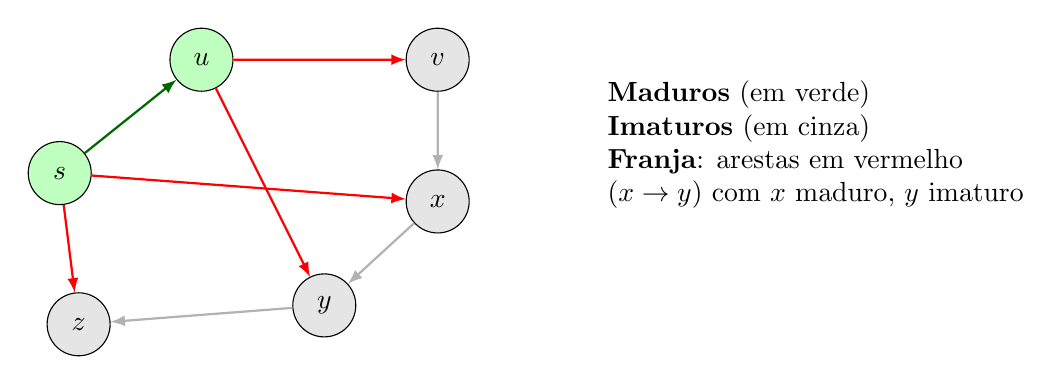
\begin{tikzpicture}[>=latex, scale=1.2]

    % estilos
    \tikzstyle{mature}=[circle, draw, fill=green!25, minimum size=8mm]
    \tikzstyle{immature}=[circle, draw, fill=gray!20, minimum size=8mm]
    \tikzstyle{franja}=[->, thick, red]
    \tikzstyle{normal}=[->, thick]

    % vértices maduros
    \node[mature] (s) at (0,0) {$s$};
    \node[mature] (u) at (1.5,1.2) {$u$};

    % vértices imaturos
    \node[immature] (v) at (4,1.2) {$v$};
    \node[immature] (x) at (4,-0.3) {$x$};
    \node[immature] (y) at (2.8,-1.4) {$y$};
    \node[immature] (z) at (0.2,-1.6) {$z$};

    % arestas normais (não franja)
    \draw[normal,gray!60] (v) -- (x);
    \draw[normal,gray!60] (x) -- (y);
    \draw[normal,gray!60] (y) -- (z);

    % arestas da franja (maduro -> imaturo)
    \draw[franja] (s) -- (x);
    \draw[franja] (s) -- (z);
    \draw[franja] (u) -- (v);
    \draw[franja] (u) -- (y);

    % aresta madura-madura
    \draw[normal, green!40!black] (s) -- (u);

    % legenda
    \node[align=left] at (8,0.3) {
        \textbf{Maduros} (em verde) \\
        \textbf{Imaturos} (em cinza) \\
        \textbf{Franja}: arestas em vermelho \\
        $(x \to y)$ com $x$ maduro, $y$ imaturo
    };

\end{tikzpicture}
\caption{A franja de um conjunto de vértices maduros na execução do algoritmo de Dijkstra.}
\label{fig:franja}
\end{figure}


\subsection*{Ideia geral do algoritmo}

Com esses conceitos em mãos, podemos descrever o algoritmo de Dijkstra da seguinte forma:

\begin{enumerate}
    \item Inicialize $dist[s] = 0$ e $dist[v] = \infty$ para todo $v \neq s$.  
          Inicialize $pai[v] = -1$ para todos os vértices e marque todos como \textbf{imaturos}.
    \item Enquanto houver vértices imaturos alcançáveis a partir de $s$:
    \begin{enumerate}
        \item escolha o vértice imaturo $y$ com menor valor de $dist[y]$ (isto é, o vértice mais próximo da árvore atual);
        \item declare $y$ \textbf{maduro}: a aresta $(pa[y],y)$ entra na árvore de caminhos mínimos (para $y=s$, temos $pa[s]=s$);
        \item para cada aresta $(y \to z)$, aplique o relaxamento:
        \[
        \text{se } dist[z] > dist[y] + w(y,z)\text{, então } dist[z] := dist[y] + w(y,z),\ pai[z] := y.
        \]
        Isso atualiza as estimativas dos vértices imaturos e, portanto, atualiza a franja.
    \end{enumerate}
\end{enumerate}

A implementação eficiente usa uma \textbf{fila de prioridade} para manter os vértices imaturos ordenados pelos valores de $dist[v]$.  
Essa fila é, na prática, uma forma compacta de representar e manipular a franja.

\subsection*{Implementação}

A seguir apresentamos uma implementação completa, compatível com a interface \texttt{Graph} e com o TAD de fila de prioridade \texttt{PQ}:

\begin{lstlisting}[language=C]
void Djikstra( Graph G, vertex s,
                 vertex *pa, int *dist)
{
   bool mature[1000];

   for (vertex v = 0; v < G->V; ++v)
      pai[v] = -1, mature[v] = false, dist[v] = INT_MAX;

   pai[s] = s;
   dist[s] = 0;

   PQinit(G->V);
   for (vertex v = 0; v < G->V; ++v)
      PQinsert(v, dist);

   while (!PQempty()) {
      vertex y = PQdelmin(dist);
      if (dist[y] == INT_MAX) break;

      for (link a = G->adj[y]; a != NULL; a = a->next) {
         if (mature[a->w]) continue;
         if (dist[y] + a->c < dist[a->w]) {
            dist[a->w] = dist[y] + a->c;
            PQdec(a->w, dist);
            pai[a->w] = y;
         }
      }
      mature[y] = true;
   }
   PQfree();
}
\end{lstlisting}

\subsection*{Por que funciona}

Com pesos não negativos, no momento em que um vértice $y$ é escolhido como o de menor $dist[y]$ entre todos os imaturos, nenhum caminho futuro poderá chegar em $y$ com custo menor.  
Portanto, a estimativa $dist[y]$ é definitiva, e $y$ pode ser marcado como \textbf{maduro}.  
Repetindo esse processo, construímos a árvore de caminhos mínimos completa.

\begin{figure}[h]
\centering
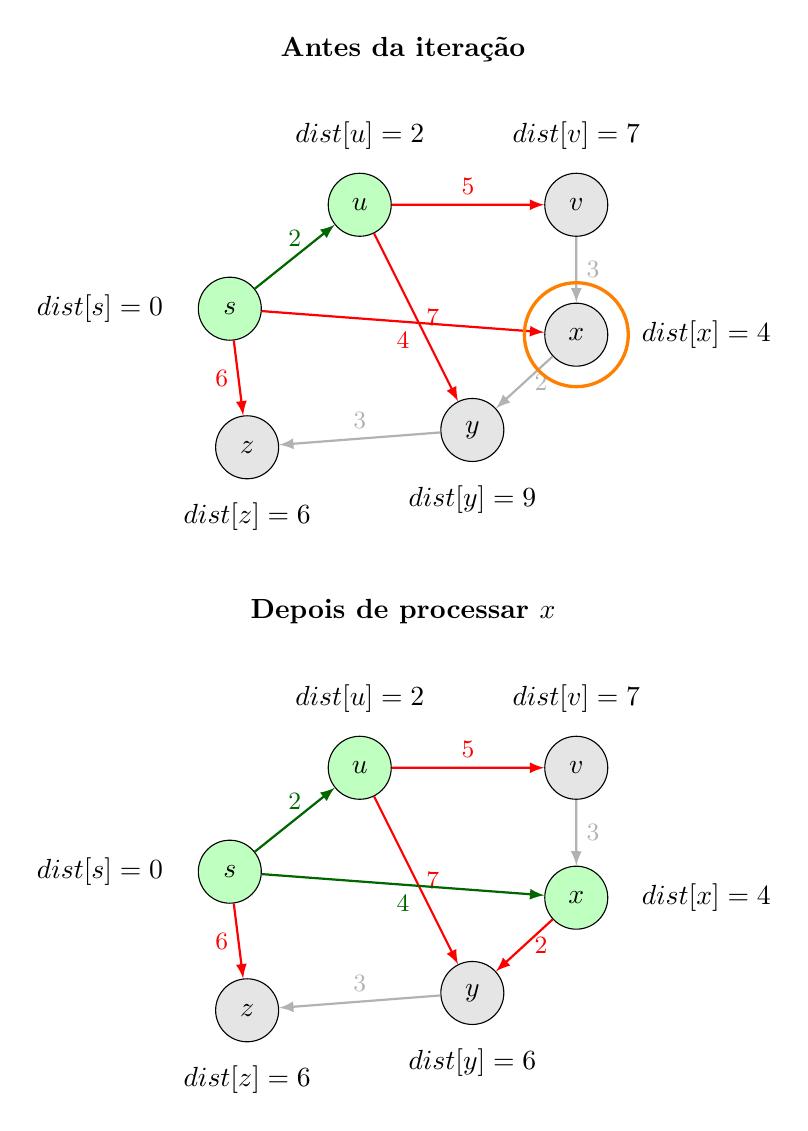
\begin{tikzpicture}[>=latex, scale=1.1]

    % estilos
    \tikzstyle{mature}=[circle, draw, fill=green!25, minimum size=8mm]
    \tikzstyle{immature}=[circle, draw, fill=gray!20, minimum size=8mm]
    \tikzstyle{franja}=[->, thick, red]
    \tikzstyle{normal}=[->, thick]

    %======================= ANTES =======================
    \begin{scope}
      \node at (2,3) {\textbf{Antes da iteração}};

      % vértices maduros
      \node[mature]   (s1) at (0,0) {$s$};
      \node[mature]   (u1) at (1.5,1.2) {$u$};

      % vértices imaturos
      \node[immature] (v1) at (4,1.2) {$v$};
      \node[immature] (x1) at (4,-0.3) {$x$};
      \node[immature] (y1) at (2.8,-1.4) {$y$};
      \node[immature] (z1) at (0.2,-1.6) {$z$};

      % arestas normais (não franja) com pesos
      \draw[normal,gray!60] (v1) -- node[right] {\small 3} (x1);
      \draw[normal,gray!60] (x1) -- node[right] {\small 2} (y1);   % x->y = 2
      \draw[normal,gray!60] (y1) -- node[above]  {\small 3} (z1);

      % arestas da franja (maduro -> imaturo) com pesos
      \draw[franja] (s1) -- node[below] {\small 4} (x1);           % s->x = 4
      \draw[franja] (s1) -- node[left]  {\small 6} (z1);           % s->z = 6
      \draw[franja] (u1) -- node[above] {\small 5} (v1);           % u->v = 5
      \draw[franja] (u1) -- node[right] {\small 7} (y1);           % u->y = 7

      % aresta maduro-maduro com peso
      \draw[normal, green!40!black] (s1) -- node[above] {\small 2} (u1); % s->u = 2

      % rótulos dist[]
      \node at (-1.5,0)   {$dist[s]=0$};
      \node at (1.5,2.0)  {$dist[u]=2$};
      \node at (4,2.0)    {$dist[v]=7$};
      \node at (5.5,-0.3) {$dist[x]=4$};
      \node at (2.8,-2.2) {$dist[y]=9$};
      \node at (0.2,-2.4) {$dist[z]=6$};

      % destaque do próximo vértice a ser escolhido (x)
      \draw[very thick, orange] (x1) circle [radius=0.6];
    \end{scope}

    %======================= DEPOIS =======================
    \begin{scope}[yshift=-6.5cm]
      \node at (2,3) {\textbf{Depois de processar $x$}};

      % vértices maduros (agora s, u e x)
      \node[mature] (s2) at (0,0) {$s$};
      \node[mature] (u2) at (1.5,1.2) {$u$};
      \node[mature] (x2) at (4,-0.3) {$x$};

      % vértices ainda imaturos
      \node[immature] (v2) at (4,1.2) {$v$};
      \node[immature] (y2) at (2.8,-1.4) {$y$};
      \node[immature] (z2) at (0.2,-1.6) {$z$};

      % arestas normais com pesos
      \draw[normal,gray!60] (v2) -- node[right] {\small 3} (x2);
      \draw[normal,gray!60] (y2) -- node[above]  {\small 3} (z2);

      % arestas da franja (maduro -> imaturo), já com x maduro
      \draw[franja] (s2) -- node[left]  {\small 6} (z2);
      \draw[franja] (u2) -- node[above] {\small 5} (v2);
      \draw[franja] (u2) -- node[right] {\small 7} (y2);
      \draw[franja] (x2) -- node[right] {\small 2} (y2);  % nova candidata via x

      % arestas maduro-maduro
      \draw[normal, green!40!black] (s2) -- node[above] {\small 2} (u2);
      \draw[normal, green!40!black] (s2) -- node[below] {\small 4} (x2);

      % rótulos dist[] atualizados
      \node at (-1.5,0)   {$dist[s]=0$};
      \node at (1.5,2.0)  {$dist[u]=2$};
      \node at (4,2.0)    {$dist[v]=7$};
      \node at (5.5,-0.3) {$dist[x]=4$};
      \node at (2.8,-2.2) {$dist[y]=6$};  % atualizado via x
      \node at (0.2,-2.4) {$dist[z]=6$};

    \end{scope}

\end{tikzpicture}
\caption{Um passo do algoritmo de Dijkstra: o vértice imaturo $x$ com menor $dist[x]$ é escolhido, torna-se maduro e suas arestas de saída são relaxadas, atualizando as estimativas dos vértices imaturos e a franja.}
\label{fig:dijkstra-passo}
\end{figure}




\subsection*{Complexidade}

A eficiência do algoritmo de Dijkstra depende crucialmente da estrutura de dados usada para selecionar,
a cada passo, o vértice imaturo com menor valor de \texttt{dist[]}.  
Essa operação — escolher o próximo vértice a ser tornado maduro — é realizada por uma
\textbf{fila de prioridade} (\textit{priority queue}), normalmente implementada como um \textbf{heap mínimo}.

\medskip

\noindent
\textbf{Heap mínimo.}  
Um heap é uma árvore binária quase completa armazenada em um vetor, na qual:

\[
\text{chave(pai)} \le \text{chave(filho)}.
\]

Assim, o menor elemento está sempre na raiz do heap e pode ser acessado em tempo $O(1)$.

O heap precisa oferecer três operações fundamentais que usamos no Dijkstra:

\begin{itemize}
    \item \textbf{delmin}: remover e retornar o vértice com menor \texttt{dist[v]};  
          \hfill custo: $O(\log |V|)$
    \item \textbf{dec}: atualizar a chave de um vértice quando seu valor \texttt{dist[v]} diminui;  
          \hfill custo: $O(\log |V|)$
    \item \textbf{insert}: inserir todos os vértices no heap no início da execução;  
          \hfill custo total: $O(|V|)$ se usado \textit{heapify}, ou $O(|V|\log|V|)$ se feito item a item
\end{itemize}

Essas operações exigem que cada vértice conheça sua posição atual no heap, para que a operação
\texttt{PQdec(v)} possa reposicioná-lo em tempo logarítmico. 
Assumimos que a implementação da fila de prioridade mantém esse mapeamento.

\medskip

\noindent
\textbf{Contagem das operações.}

Durante a execução do algoritmo:

\begin{itemize}
    \item Cada vértice é removido da fila \emph{exatamente uma vez} por \texttt{PQdelmin}.  
          São $|V|$ remoções, cada uma custando $O(\log |V|)$.
    \item Cada aresta pode causar no máximo \emph{uma} chamada bem-sucedida a \texttt{PQdec},  
          pois cada relaxamento bem-sucedido reduz a distância de um vértice uma única vez.  
          São no máximo $|E|$ chamadas, cada uma custando $O(\log |V|)$.
\end{itemize}

Somando esses custos:

\[
O(|V|\log|V|) \;+\; O(|E|\log|V|) \;=\; O(|E|\log|V|).
\]

\medskip


\section{Algoritmo de Bellman--Ford}

O algoritmo de Bellman--Ford resolve o problema dos caminhos mínimos a partir de uma origem $s$
mesmo quando o grafo possui arestas de peso negativo.
Além disso, o algoritmo é capaz de detectar a existência de ciclos de custo negativo
alcançáveis a partir de $s$.

Ao contrário do Dijkstra, o Bellman--Ford \textbf{não usa franja}
e \textbf{não pressupõe} que as estimativas se tornam definitivas
à medida que o algoritmo progride.
Em vez disso, ele se apoia inteiramente no \textbf{princípio do relaxamento}.

\subsection*{Ideia básica}

Um caminho simples (sem repetir vértices) possui no máximo $|V|-1$ arestas.
Portanto, se não houver ciclos negativos,
após realizar o relaxamento de \emph{todas} as arestas do grafo
\textbf{$|V|-1$ vezes},
todas as estimativas \texttt{dist[]}
terão alcançado os valores ótimos.

Após essas iterações, se ainda existir alguma aresta $(u,v)$
tal que

\[
dist[v] > dist[u] + w(u,v),
\]

então existe um ciclo negativo acessível a partir da origem.

\medskip

Essa formulação — dois laços aninhados — é a versão clássica do algoritmo.
Mas ela faz trabalho desnecessário:
relaxamos todas as arestas em todas as iterações,
mesmo que muitas delas não possam mais melhorar nada.

Uma implementação muito mais eficiente usa uma \textbf{fila} de vértices cujas estimativas acabaram de melhorar e que ainda podem melhorar os vizinhos.

\subsection*{Descrição do algoritmo}

Mantemos:

\begin{itemize}
    \item o vetor de estimativas \texttt{dist[]};
    \item o vetor de pais \texttt{pai[]};
    \item uma fila com vértices que precisam ser processados;
    \item um vetor booleano \texttt{onqueue[]} indicando se um vértice está na fila.
\end{itemize}

O algoritmo começa com apenas o vértice fonte na fila.
Sempre que uma estimativa \texttt{dist[w]} melhora,
o vértice $w$ é colocado na fila (se ainda não estiver lá).

Para controlar o número de ``rodadas'' completas de relaxamentos,
usamos um \textbf{sentinela} $V$ na fila.
A cada vez que o sentinela é retirado da fila, isso indica que uma rodada terminou.
Se fizermos $|V|$ rodadas, então existe um ciclo negativo acessível.

\subsection*{Implementação}

\begin{lstlisting}[language=C]
bool bellmannFord( Graph G, vertex s, vertex *pa, int *dist)
{
   QUEUEinit( G->A);
   bool onqueue[1000];

   for (vertex u = 0; u < G->V; ++u)
      pa[u] = -1, dist[u] = INT_MAX, onqueue[u] = false;

   pa[s] = s;
   dist[s] = 0;

   QUEUEput( s );
   onqueue[s] = true;

   vertex V = G->V;     // pseudovértice sentinela
   QUEUEput( V );       // marca o fim da primeira rodada

   int k = 0;           // número de rodadas realizadas

   while (true) { 
      vertex v = QUEUEget();

      if (v < V) {      // v é vértice real
         for (link a = G->adj[v]; a != NULL; a = a->next) {
            if (dist[v] + a->c < dist[a->w]) {
               dist[a->w] = dist[v] + a->c; 
               pa[a->w] = v;
               if (!onqueue[a->w]) {
                  QUEUEput( a->w );
                  onqueue[a->w] = true;
               }
            }
         }
      } 
      else {            // encontramos o sentinela
         if (QUEUEempty())
            return true;   // nenhuma melhora possível: sucesso

         if (++k >= G->V)
            return false;  // ciclo negativo detectado

         QUEUEput( V );    // prepara a próxima rodada
         for (vertex u = 0; u < G->V; ++u)
            onqueue[u] = false;
      }
   }
}
\end{lstlisting}

\subsection*{Corretude}

Se não houver ciclos negativos, então o algoritmo executa no máximo $|V|-1$ rodadas de relaxamento global, e todas as distâncias finais serão ótimas.

Se houver um ciclo negativo alcançável, então as estimativas continuarão melhorando indefinidamente, o sentinela será removido da fila ao menos $|V|$ vezes e o algoritmo detectará isso pelo contador $k$.

\subsection*{Complexidade}

No algoritmo com fila, um vértice $v$ entra na fila sempre que sua estimativa \texttt{dist[v]} diminui.
Em grafos sem ciclos negativos, a distância de um vértice pode melhorar no máximo $|V|-1$ vezes, pois um caminho simples possui no máximo $|V|-1$ arestas.

Cada vez que um vértice é retirado da fila, percorremos todas as arestas que saem dele, realizando possíveis relaxamentos.  
Assim, no pior caso, cada vértice pode ser processado até $|V|-1$ vezes, e cada processamento
examinará seu leque de saída:

\[
O((|V|-1)\cdot |E|) = O(|V||E|).
\]

\medskip

\noindent
\textbf{Observação.}
Esse pior caso é raro.
Na maioria dos grafos, as estimativas \texttt{dist[]} estabilizam rapidamente, e apenas poucos vértices entram na fila.
Quando isso ocorre, o número de relaxamentos executados é muito menor que $|V||E|$, tornando o algoritmo substancialmente mais rápido na prática.


\section{Comparação entre Dijkstra e Bellman--Ford}

\begin{table}[h]
\centering
\begin{tabular}{|l|c|c|}
\hline
\textbf{Característica} & \textbf{Dijkstra} & \textbf{Bellman--Ford} \\ \hline
Pesos negativos & não & sim \\ \hline
Detecta ciclo negativo & não & sim \\ \hline
Estratégia & franja + heap & relaxamentos iterativos \\ \hline
Complexidade típica & $O(|E|\log|V|)$ & $O(|V||E|)$ \\ \hline
Estrutura usada & fila de prioridade (heap) & fila comum \\ \hline
\end{tabular}
\end{table}
